% !TeX root = ../../thesis.tex
\chapter{Aims and objectives}\label{ch:objective}

This chapter is dedicated to the elaboration of the objectives of the current thesis. It starts with the general definition of the doctoral project aims. Hereafter, the specific objectives of the doctoral project are demonstrated. Then, the chapter illustrates the thesis's outline and structure.


\section{General aim}


The use of biodegradable metals has been gaining attention for various kinds of biomedical applications in recent decades, however, controlling their functionality and behavior inside the body has remained a challenge. Computational modeling of the materials’ interaction with the body can help avoid part of the expensive experimental works required to characterize the degradation properties and can provide an integrated spatiotemporal view of the whole process.

One of the most challenging parts of performing such a modeling study is to capture the chemical interactions and the dynamics and kinetics of the reactions occurring on the material-environment interface. Taking advantage of mechanistic modeling principles of mass transfer coupled with free boundary and moving interface formulations seems to be a promising solution to this complex problem. By doing so, one can model the degradation process by a set of equations capturing the interaction of various chemical components while tracking the moving corrosion front, which changes the location where the dynamic is taking place.

In this study, we have developed a mathematical and computational model to predict the biodegradation behavior of biodegradable metallic biomaterials, focusing on Mg. This model enables us to investigate the chemical and, later on, biological phenomena occurring on the corrosion interface of these biomaterials. Additionally, coupling the model with other existing cell and tissue growth models leads to a multiphysics model combining the chemistry of biodegradation, the physics of the electrolytes and body fluids flow, and the biology of tissue growth/regeneration. Building such a model requires dealing with several challenges, one of which is to couple various functions used to track the moving boundary of different sub-problems. Moreover, adding the effect of convection imposed by the fluid flow increases the system's complexity. Elaborating these challenges from a mathematical point of view will facilitate future contributions to constructing such models.


\section{Specific objectives} \label{sec:aim_objective}

Despite the advantages of using biodegradable metals in implant design, their fast degradation and uncontrolled release remain a challenge in practical applications. A validated computational model of the degradation process can facilitate the tuning of biodegradation properties. In this doctoral project, a physicochemical model was developed by deriving a mathematical model of the chemistry of biodegradation of Mg and implementing its 3D computational model using the finite element method. To accomplish this, the project was divided into five main objectives, illustrated schematically in Fig. \ref{fig:objective_project_outline}.

\begin{figure}
\centering
\medskip
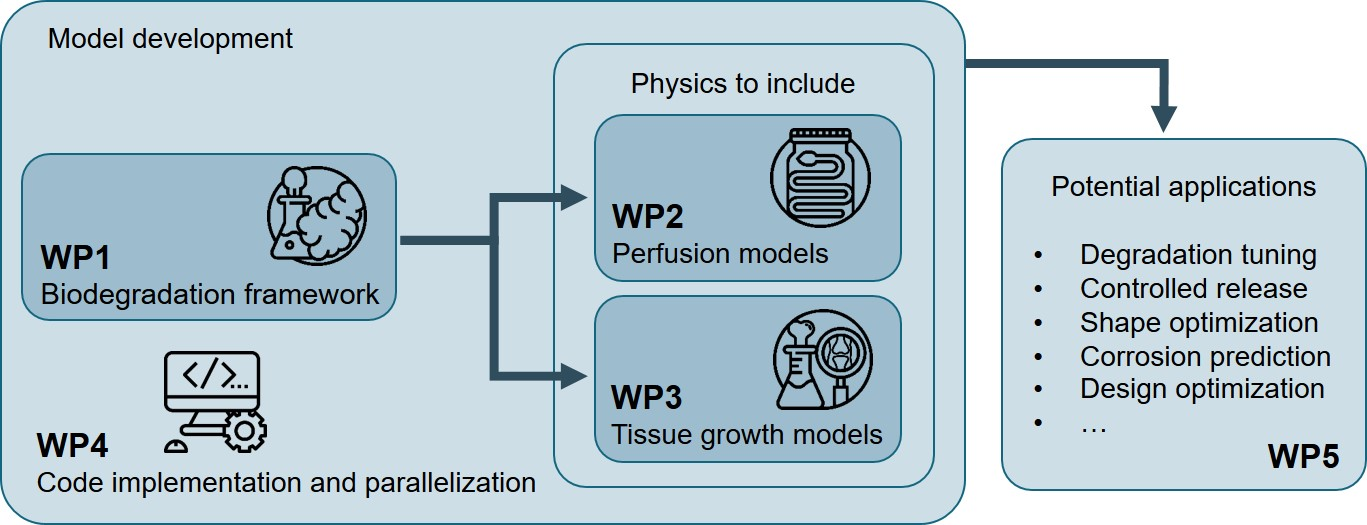
\includegraphics[width=1.0\textwidth]{project_outline.jpg}
\caption[Schematic of the project outline]{Schematic representation of the structure and outline of the current project, divided into five objectives.} \label{fig:objective_project_outline}
\end{figure}

\textbf{Objective 1} was with the development of the core biodegradation model. For this purpose, a physicochemical model of the biodegradation process of commercially-pure Mg was developed by constructing a mathematical model formulating the mass transfer phenomena and tracking the location of the implant's surface during degradation. For the mass transfer model, a set of time-dependent reaction-diffusion-convection partial differential equations were derived from the chemistry of biodegradation of the Mg in saline (NaCl) and buffered (\gls{SBF}) solutions, which usually includes the oxidation of the metallic part, reduction of water and oxygen, changes in local and global pH, and formation of a protective film on the surface of the scaffold which contributes to a slower rate of degradation. Besides these aspects, it was also crucial to consider the effect of different ions in the medium on the degradation rate. Additionally, investigating the structural changes of the scaffolds and implants in practical applications like the resorption of temporary fixation devices, requires tracking the movement of the corrosion surface. This was done by constructing an equation based on the level-set principle, which captured the movement of the medium-metal interface by defining an implicit surface. The derived equations were coupled and solved using the finite element method. The degradation data to validate the models were collected from immersion tests. The model parameters were calibrated using a Bayesian optimization algorithm, and the obtained parameters were used to simulate the pH changes in NaCl and \gls{SBF} solutions.

\textbf{Objective 2} was the coupling of corresponding equations of fluid flow (Navier-Stokes and Stokes equations) in the solution domain with the biodegradation model to capture the effect of convection on the degradation process. This was crucial in order to consider the conditions in perfusion bioreactors and hydrodynamics experiments. The main challenge for this step was the complexity of dealing with the finite element formulation of fluid flow equations and the difficulty of defining proper fluid boundary conditions on an implicit interface (the corrosion front).

The \textbf{third objective} was to couple the degradation model with the tissue growth models to simulate the response of the surrounding tissue during the biodegradation process. For doing this, a detailed tissue growth model was developed using two different interface tracking techniques, the phase-field and level-set methods, and the results and efficiency of both methods were compared. The mathematical coupling of the degradation and tissue growth models and validating their predictions remained a challenge in this work package.

The \textbf{fourth objective} was related to the optimization of the computational aspects of the thesis with  all the codes developed in-house using open-source tools and libraries. Detailed work on the parallelization of the computational models of the three previous objectives was carried out to make the developed models run faster. As the required high accuracy on the moving interface increases computation time, parallelization was crucial for the computational models to decrease the execution time of the simulations. The parallel algorithm was implemented using a domain decomposition method. Besides this, the formed linear system of equations in each partition of the mesh was solved using Krylov methods by taking advantage of available highly efficient preconditioners and iterative solvers, and the scaling behavior with respect to the available computational resources was measured for different components of the models.

The \textbf{fifth objective} was the demonstration of the versatility of the developed model  by using it as the biodegradation compartment in several multiphysics  use-cases to demonstrate the ability of the model to be integrated into other modeling workflows for biomedical applications. In the performed studies, the biodegradation model was combined with structural mechanics and topology optimization codes to deliver a more comprehensive model of the underlying phenomena. The case studies presented in this thesis include mechanical loosening of mandibular bone plates, degradation of an optimized acetabular cup implant, and mechanical integrity of infilled structures.


\section{Thesis outline}

The objectives mentioned in Section \ref{sec:aim_objective} are tackled in the chapters ahead in the following order and structure:

\textbf{Chapters \ref{ch:core} and \ref{ch:kinetics}} describe the development of the core biodegradation model of \textbf{Objective 1}. In \textbf{Chapter \ref{ch:core}}, a basic biodegradation model is described, which is the base for combining the model with more physics in different applications. \textbf{Chapter \ref{ch:kinetics}} further develops the base model to include more advanced chemistry from the biodegradation of Mg in more complex electrolytes and conditions.

\textbf{Chapter \ref{ch:fluid}} describes the development of the fluid flow model used for the simulation of hydrodynamics conditions, which is related to \textbf{Objective 2} for coupling the biodegradation model with flow problems. The output coupled model is later used in \textbf{Chapter \ref{ch:kinetics}} for validating the biodegradation model in hydrodynamics conditions.

The work presented in \textbf{Chapter \ref{ch:tissue}} is related to \textbf{Objective 3}, in which a tissue growth model is developed to be coupled with the biodegradation model. A simplified tissue growth model is also developed and used in \textbf{Chapter \ref{ch:mandible}}, where the rate of bone healing is modeled during the degradation of a mandibular plate, leading to loss of mechanical strength.

Works related to \textbf{Objective 4} are presented in \textbf{Chapters \ref{ch:hpc}, \ref{ch:biodeg}, and \ref{ch:bayesian}}, in which the details of software development and model parallelization are elaborated. \textbf{Chapter \ref{ch:hpc}} discusses the steps and details of parallelization of the implemented biodegradation model, which can be generalized as a free boundary problem coupled with reaction-diffusion systems. As part of this work package, the developed biodegradation model was transformed into a multifunctional 3D code called BioDeg, the details of which are described in \textbf{Chapter \ref{ch:biodeg}}. Additionally, the workflow and routines used to calibrate the models and estimate the unknown parameters are presented in \textbf{Chapter \ref{ch:bayesian}}, which were also published as educational materials. Furthermore, some parallel scaling behavior results and discussion of the biodegradation model are presented in \textbf{Chapter \ref{ch:cup}}.

In the end, \textbf{Chapters \ref{ch:cup}, \ref{ch:infill}, and \ref{ch:mandible}} are related to \textbf{Objective 5}, dedicated to demonstrating some of the applications of the developed biodegradation model. \textbf{Chapter \ref{ch:cup}} presents the work done to combine the degradation model with the output of a surrogate model, in which the degradation behavior of a patient-specific porous acetabular implant was investigated. \textbf{Chapter \ref{ch:infill}} describes the coupling of the degradation model with a topology optimization code, in which the change of stiffness of some infilled structures was modeled during the degradation process. Lastly, in \textbf{Chapter \ref{ch:mandible}}, the biodegradation model was used to predict the rate of mass loss for a mandibular plate, which was subsequently converted to a mechanical strength analysis model to examine how the plate characteristics react to degradation. 

To facilitate the structure of the thesis, the chapters related to \textbf{Objectives one to three} are grouped in \textbf{Part 2} ``Model Development'', the chapters related to \textbf{Objective 4} are presented in \textbf{Part 3} ``Code Implementation and Software Development'', and the chapters related to \textbf{Objective 5} are presented in \textbf{Part 4} ``Model Applications''.

%%%%%%%%%%%%%%%%%%%%%%%%%%%%%%%%%%%%%%%%%%%%%%%%%%
% Keep the following \cleardoublepage at the end of this file,
% otherwise \includeonly includes empty pages.
\cleardoublepage
